\section{Kasutaja tagasiside}

Tööle küsiti tagasisidet Tallinna 21. Kooli arengujuhilt, kellel paluti süsteemi kasutada ilma abita. Tagasiside saamise eesmärk oli näha kui lihtne on rakendust kasutada ning mida saaks rakenduses parandada.

Kasutajal oli rakendust kasutades raskus leida üles ülesannete vastused. Peale töö loomist ja salvestamist ei suunatud kasutajat kuhugi edasi, mis võis tekitada temas segadust. Töö genereerimise vaates oli küll kuvatud töö variandid, kuid puudus vastuseleht.

Kasutaja ei saanud aru rakenduses oleva malli põhimõttest. Rakendus ei selgitanud kasutajale piisavalt hästi malli tähendust ja kuidas see on seotud genereeritavate töödega.

Kasutaja soovis, et rakenduses oleks võimalik luua rohkem ülesandeid, mis oleksid sobilikud kümnenda klassi õpilastele. Rakenduses oli tagasiside saamise hetkel ainult kolm ülesandetüüpi, mis ei kataks suurt osa kümnenda klassi matemaatika õppekavas olevatest teemadest.

Tagasiside andja oli projektist huvitatud ning soovis seda võimalusel kasutusele võtta peale seda kui õpetajad on saanud rakendust proovida.

\section{Täiustused}

Tagasiside põhjal tehti töös muudatusi, et parandada rakenduse kasutamise kogemust.

Selleks, et loodud töid ja nendega seotud vastuseid oleks lihtsam leida, loodi teatesõnum, mida kuvatakse peale töö genereerimist. Teatesõnumit näidatakse vaate päises ning seda vajutades suunatakse kasutaja töö detailvaatesse, kus saab eraldi avada erinevaid töö variante ning tööga seotud vastuselehte. Lisati ka töö genereerimise vaatesse võimalus kuvada vastuselehte, et vastused oleks kohe näha enne töö salvestamist. Joonis \ref{fig:test-generation-save-view-notification} kuvab töö salvestamise vaadet koos teatesõnumiga ja lisatud vastuselehega.

Lisaks muudele täiustustele lisati rakendusele ka tagasiside andmise vorm. Vorm on saadaval rakenduse päises oleva nupu all ning seda vajutades suunatakse kasutaja tagasiside andmise vaatesse. Vaates on tekstikast, kuhu kasutaja saab soovitud tagasiside kirjutada, ning nupp tagasiside saatmiseks.

Täiustuste tegemise käigus ei lisatud ajaliste piirangute tõttu võimalusi genereerida ülesandetüüpe, mis käsitleks kümnenda klassi matemaatika teemasid.

\begin{figure}[H]
    \centering
    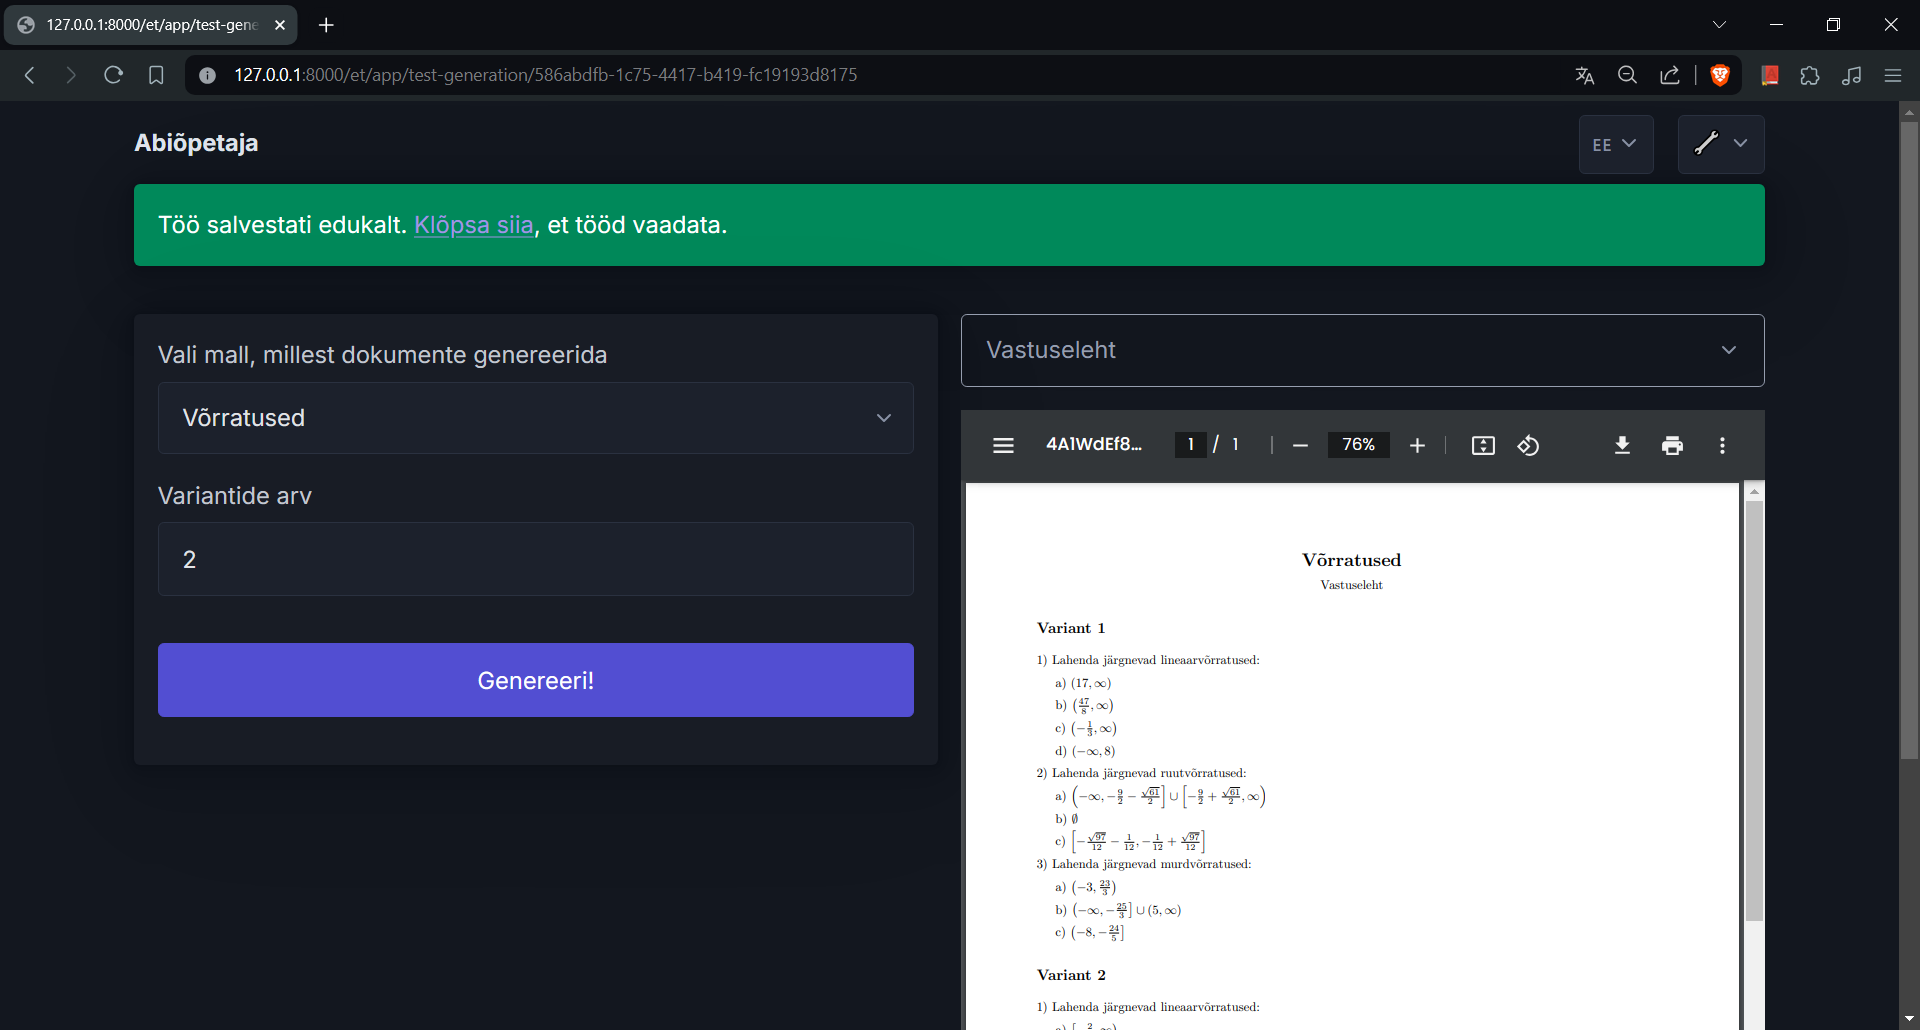
\includegraphics[width=\textwidth]{test_generation_save_view_notification}
    \caption{\emph{Töö salvestamise vaade koos teatesõnumiga.}}
    \label{fig:test-generation-save-view-notification}
\end{figure}
